%----------------------------------------------------------------------------------------
%	SECTION 1.4
%----------------------------------------------------------------------------------------

\section{The Product Topology.}

\begin{definition}
    Let $X$ and $Y$ be topological spaces. We define the \textbf{product topology} on
    $X \times Y$ to be the topology having as basis the collection
    \begin{equation*}
\Bc=\{U \times V \subseteq X \times Y:
    U \text{ is open in } X \text{ and } V \text{ is open in } Y\}
    \end{equation*}
\end{definition}

\begin{theorem}\label{1.4.1}
    The collection $\Bc=\{U \times V \subseteq X \times Y: U \text{ is open in }
        X \text{ and } V \text{ is open in } Y\}$ forms a basis for the product
        topology on $X \times Y$.
\end{theorem}
\begin{proof}
    Clearly, we have that $X \times Y$ is a basis element of  $\Bc$. Now take
    $U_1 \times V_1$ and $U_2 \times V_2$ in $\Bc$. Since  $U_1 \times V_1
    \cap U_2 \times V_2=U_1 \cap U_2 \times V_1 \cap V_2$, since $U_1 \cap U_2$
    and $V_1 \cap V_2$ are open in $X$ and  $Y$ respectively, then we have that
    $U_1 \times V_1 \cap U_2 \times V_2$ is a basis element as well.
\end{proof}

\begin{theorem}\label{1.4.2}
    If $\Bc$ is the basis for a topology on  $X$, and  $\Cc$ is the basis for a
    topology on  $Y$, then the collection:
        \begin{equation*}
            \Dc=\{B \times C: B \in \Bc \text{ and } C \in \Cc\}
        \end{equation*}
    Is a basis for the topology on $X \times Y$.
\end{theorem}
\begin{proof}
    By lemma \ref{1.2.3}, let $W$ be an open set of  $X \times Y$, and let
    $x \times y \in W$. Then there is a basis  $U \times V$ such that
    $x \times y \in U \times V \subseteq W$. Since  $\Bc$ and  $\Cc$ are bases
    of  $X$ and  $Y$ respectively, choosing  $B \in \Bc$ and  $C \in \Cc$, we
    have that  $x \in B \subseteq U$, and  $y \in C \subseteq Y$, thus
    $x \times y \in B \times C \subseteq U \times V \subseteq W$. Therefore,
    $\Dc$ is the basis for a topology on  $X \times Y$.
\end{proof}

\begin{example}
    The product of the standard topology on $\R$ with itself is called the
    \textbf{standard topology on $\R \times \R$}, and has as basis the
    collection of all products of open sets in $\R$. By theorem \ref{1.4.2},
    if we take the collection of all open intervals $(a,b) \times (c,d)$ in
    $\R \times \R$, we form a basis. Constructing this basis geometrically
    gives the interior of a rectangle, whose boundaries are the intervals
    $(a,b)$ and  $(c,d)$.

    \begin{figure}[h]
        \centering
        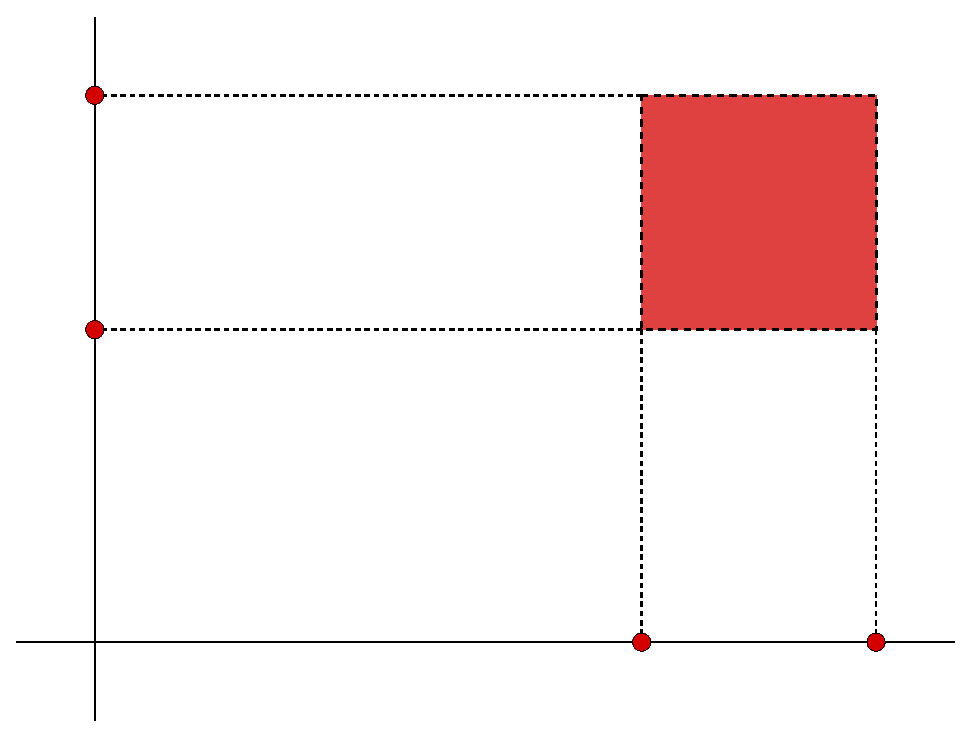
\includegraphics[scale = 0.5]{Figures/Chapter1/basis_on_RxR.eps}
        \caption{A basis element for $\R \times \R$}
        \label{fig1.4}
    \end{figure}
\end{example}

\begin{definition}
    Let $\pi_1:X \times Y \rightarrow X$ be defined such that  $\pi_1(x,y)=x$,
    and define $\pi_2:X \times Y \rightarrow Y$ such that $\pi_2(x,y)=y$. We
    call $\pi_1$ and $\pi_2$ \textbf{projections} of $X \times Y$ onto its
    first and second \textbf{factors}; that is onto $X$ and $Y$, respectively.
\end{definition}

Clearly, $\pi_1$ and $\pi_2$ are both onto. Now let $U$ be open in  $X$, then
$\pi_1^{-1}(U)=U \times Y$ is open in $X \times Y$ ; similarly,
$\pi_2^{-1}(V)=X \times V$ is also open in $X \times Y$, for  $V$ open in  $Y$.

\begin{example}\label{1.7}
    The maps $:\pi_1:x \times y \rightarrow x$ and $\pi_2:x \times y \rightarrow
    y$ of $X \times Y$ onto  $X$ and  $Y$, repsectively, are what we call ``open
    maps''. Let $U$ and  $V$ be open in  $X$ and  $Y$ respectively, then  $U
    \times V$ is open in  $X \times Y$, and for every  $x \times y \in U \times
    V$, we have  $\pi_1(x \times y)=x$ and $\pi_2(x \times y)=y$, so that
    $\pi_1(U \times V)=U$ and $\pi_2(U \times V)=V$ are open in $X$ and  $Y$
    respectively.
\end{example}

\begin{theorem}\label{1.4.3}
    The collection $\Sc=\{\pi_1^{-1}(U): U \text{ is open in } X\} \cup o
    \{\pi_2^{-1}(V): V \text{ is open in } Y\}$ is a subbasis for the product
    topology on $X$.
\end{theorem}
\begin{proof}
    Let $\Tc$ be the product topology on  $X \times Y$, and let  $\Tc'$ be the topology
    generated by $\Sc$. Since every element of  $\Sc$ is open in  $\Tc$,  $\Tc \subseteq \Tc'$. Conversely,
    consider the basis element  $U \times V$ of $\Tc$, then  $\pi_1^{-1}(U) \cap \pi_2^{-1}(V)=
    U \times Y \cap X \times V=U \times V$, thus $\Tc \subseteq \Tc'$. Therefore, $\Sc$ is a subbasis for the
    product topology.
\end{proof}

\begin{figure}[h]
    \centering
    
\includegraphics[scale = 0.5]{Figures/Chapter1/inverse_projections.eps}
    \caption{The inverse images, $\pi_1^{-1}(U)$ and $\pi_2^{-1}(V)$, of the
    projections $\pi_1$ and $\pi_2$ onto the $X \times Y$ plane.}
    \label{fig1.5}
\end{figure}
